\subsection{Allowed Ingress Traffic}

The nmap tool \cite{nmap} was used to look for open \gls{tcp} and \gls{udp} ports on the \gls{cpe} under analysis. Additionally, the ping tool \cite{ping} was also executed to check if \gls{icmp} traffic was allowed.

First, both tools were used from inside the \gls{lan} towards the \gls{cpe}’s private \gls{ip}, listing which ports were exposed to the local network. The execution of both tools is shown on Figure \ref{figure:cpe_allowed_ingress_traffic}.

\begin{figure}[h]
    \centering
    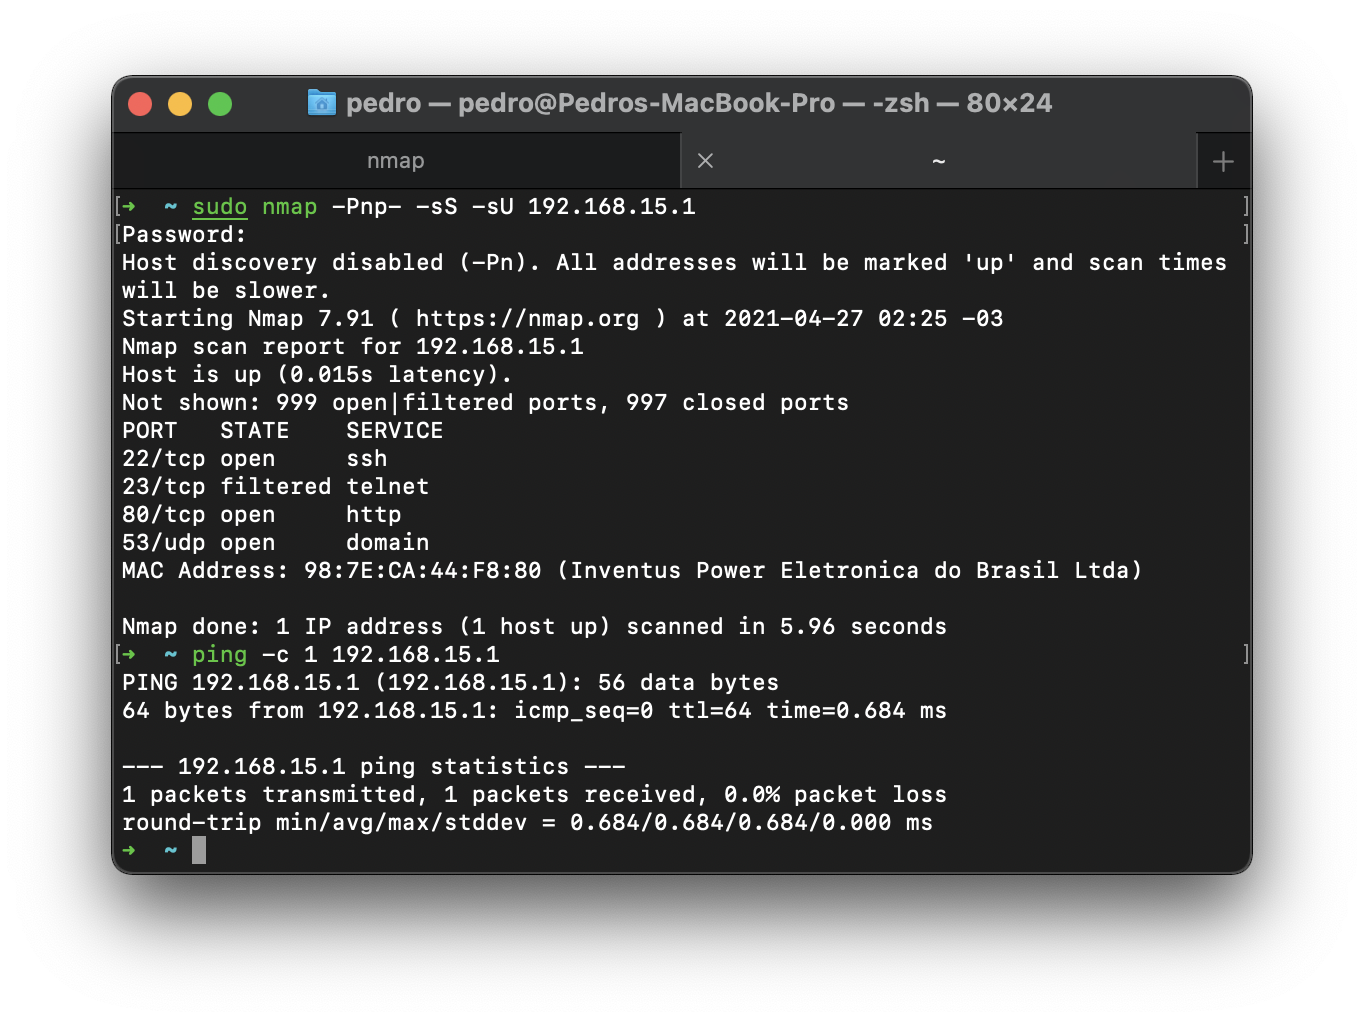
\includegraphics[width=\linewidth]{contents/cpes-and-research-data/allowed-ingress-traffic/cpe-allowed-ingress-traffic.png}
    \caption{\gls{cpe} Allowed Ingress Traffic}
    \label{figure:cpe_allowed_ingress_traffic}
\end{figure}

Then, to detect the ports exposed to the broadband network, the \gls{cpe} had to be connected to the copper or fiber cable of the \gls{isp} to acquire a public \gls{ip} address. The tools were executed from a device on the \gls{wan}, directing the scan to the \gls{cpe}’s public \gls{ip}.

Table \ref{table:cpes_ingress} presents all ingress traffic allowed by the \gls{cpe} on both \gls{lan} and \gls{wan} sides.

\begin{table}[h]
    \makebox[\linewidth]{
        \begin{tabular}{c|c|c}
            \thead{\gls{cpe} Identifier} & \thead{From \gls{lan}-side} & \thead{From \gls{wan}-side} \\
            \hline
            \gls{cpe}-0 & \texttt{53/udp 80/tcp 443/tcp 5431/tcp \gls{icmp}} & \texttt{7547/tcp \gls{icmp}} \\
            \gls{cpe}-1 & \texttt{53/udp 80/tcp 443/tcp 5431/tcp \gls{icmp}} & \texttt{7547/tcp \gls{icmp}} \\
            \gls{cpe}-2 & \texttt{22/tcp 53/udp 80/tcp \gls{icmp}} & \texttt{22/tcp 80/tcp 7547/tcp \gls{icmp}} \\
            \gls{cpe}-3 & \texttt{22/tcp 53/udp 80/tcp \gls{icmp}} & \texttt{22/tcp 80/tcp 7547/tcp \gls{icmp}} \\
            \gls{cpe}-4 & \texttt{53/udp 80/tcp \gls{icmp}} & \texttt{7547/tcp \gls{icmp}} \\
            \gls{cpe}-5 & \texttt{53/udp 80/tcp \gls{icmp}} & \texttt{7547/tcp \gls{icmp}} \\
            \gls{cpe}-6 & \texttt{80/tcp 443/tcp \gls{icmp}} & \texttt{7547/tcp \gls{icmp}} \\
            \gls{cpe}-7 & \texttt{53/udp 80/tcp 5555/tcp \gls{icmp}} & \texttt{7547/tcp \gls{icmp}} \\
        \end{tabular}
    }
    \caption{Allowed Ingress Traffic of the \gls{cpe}s}
    \label{table:cpes_ingress}
\end{table}

\FloatBarrier
